\section{FEFF9 Design}

FEFF is an \textit{ab initio} absorption simulation software based on real-space multiple scattering (RSMS) and the Greene's function. The current version, FEFF9, calculates a self-consistent density function over a wide range of structures by considering the excited state properties within an all-electron framework \cite{feff-new-dev}. Like other density-functional theory (DFT) software, FEFF begins with an initial guess for the electronic density. Then, using an optimization algorithm like gradient descent (see section \ref{sec:optimizers}), FEFF iterates through a series of calculations until the resulting potential matches the initial potential (self-consistency). This process is depicted in Figure \ref{fig:feff-dft-diagram}.

\begin{figure}
    \centering
    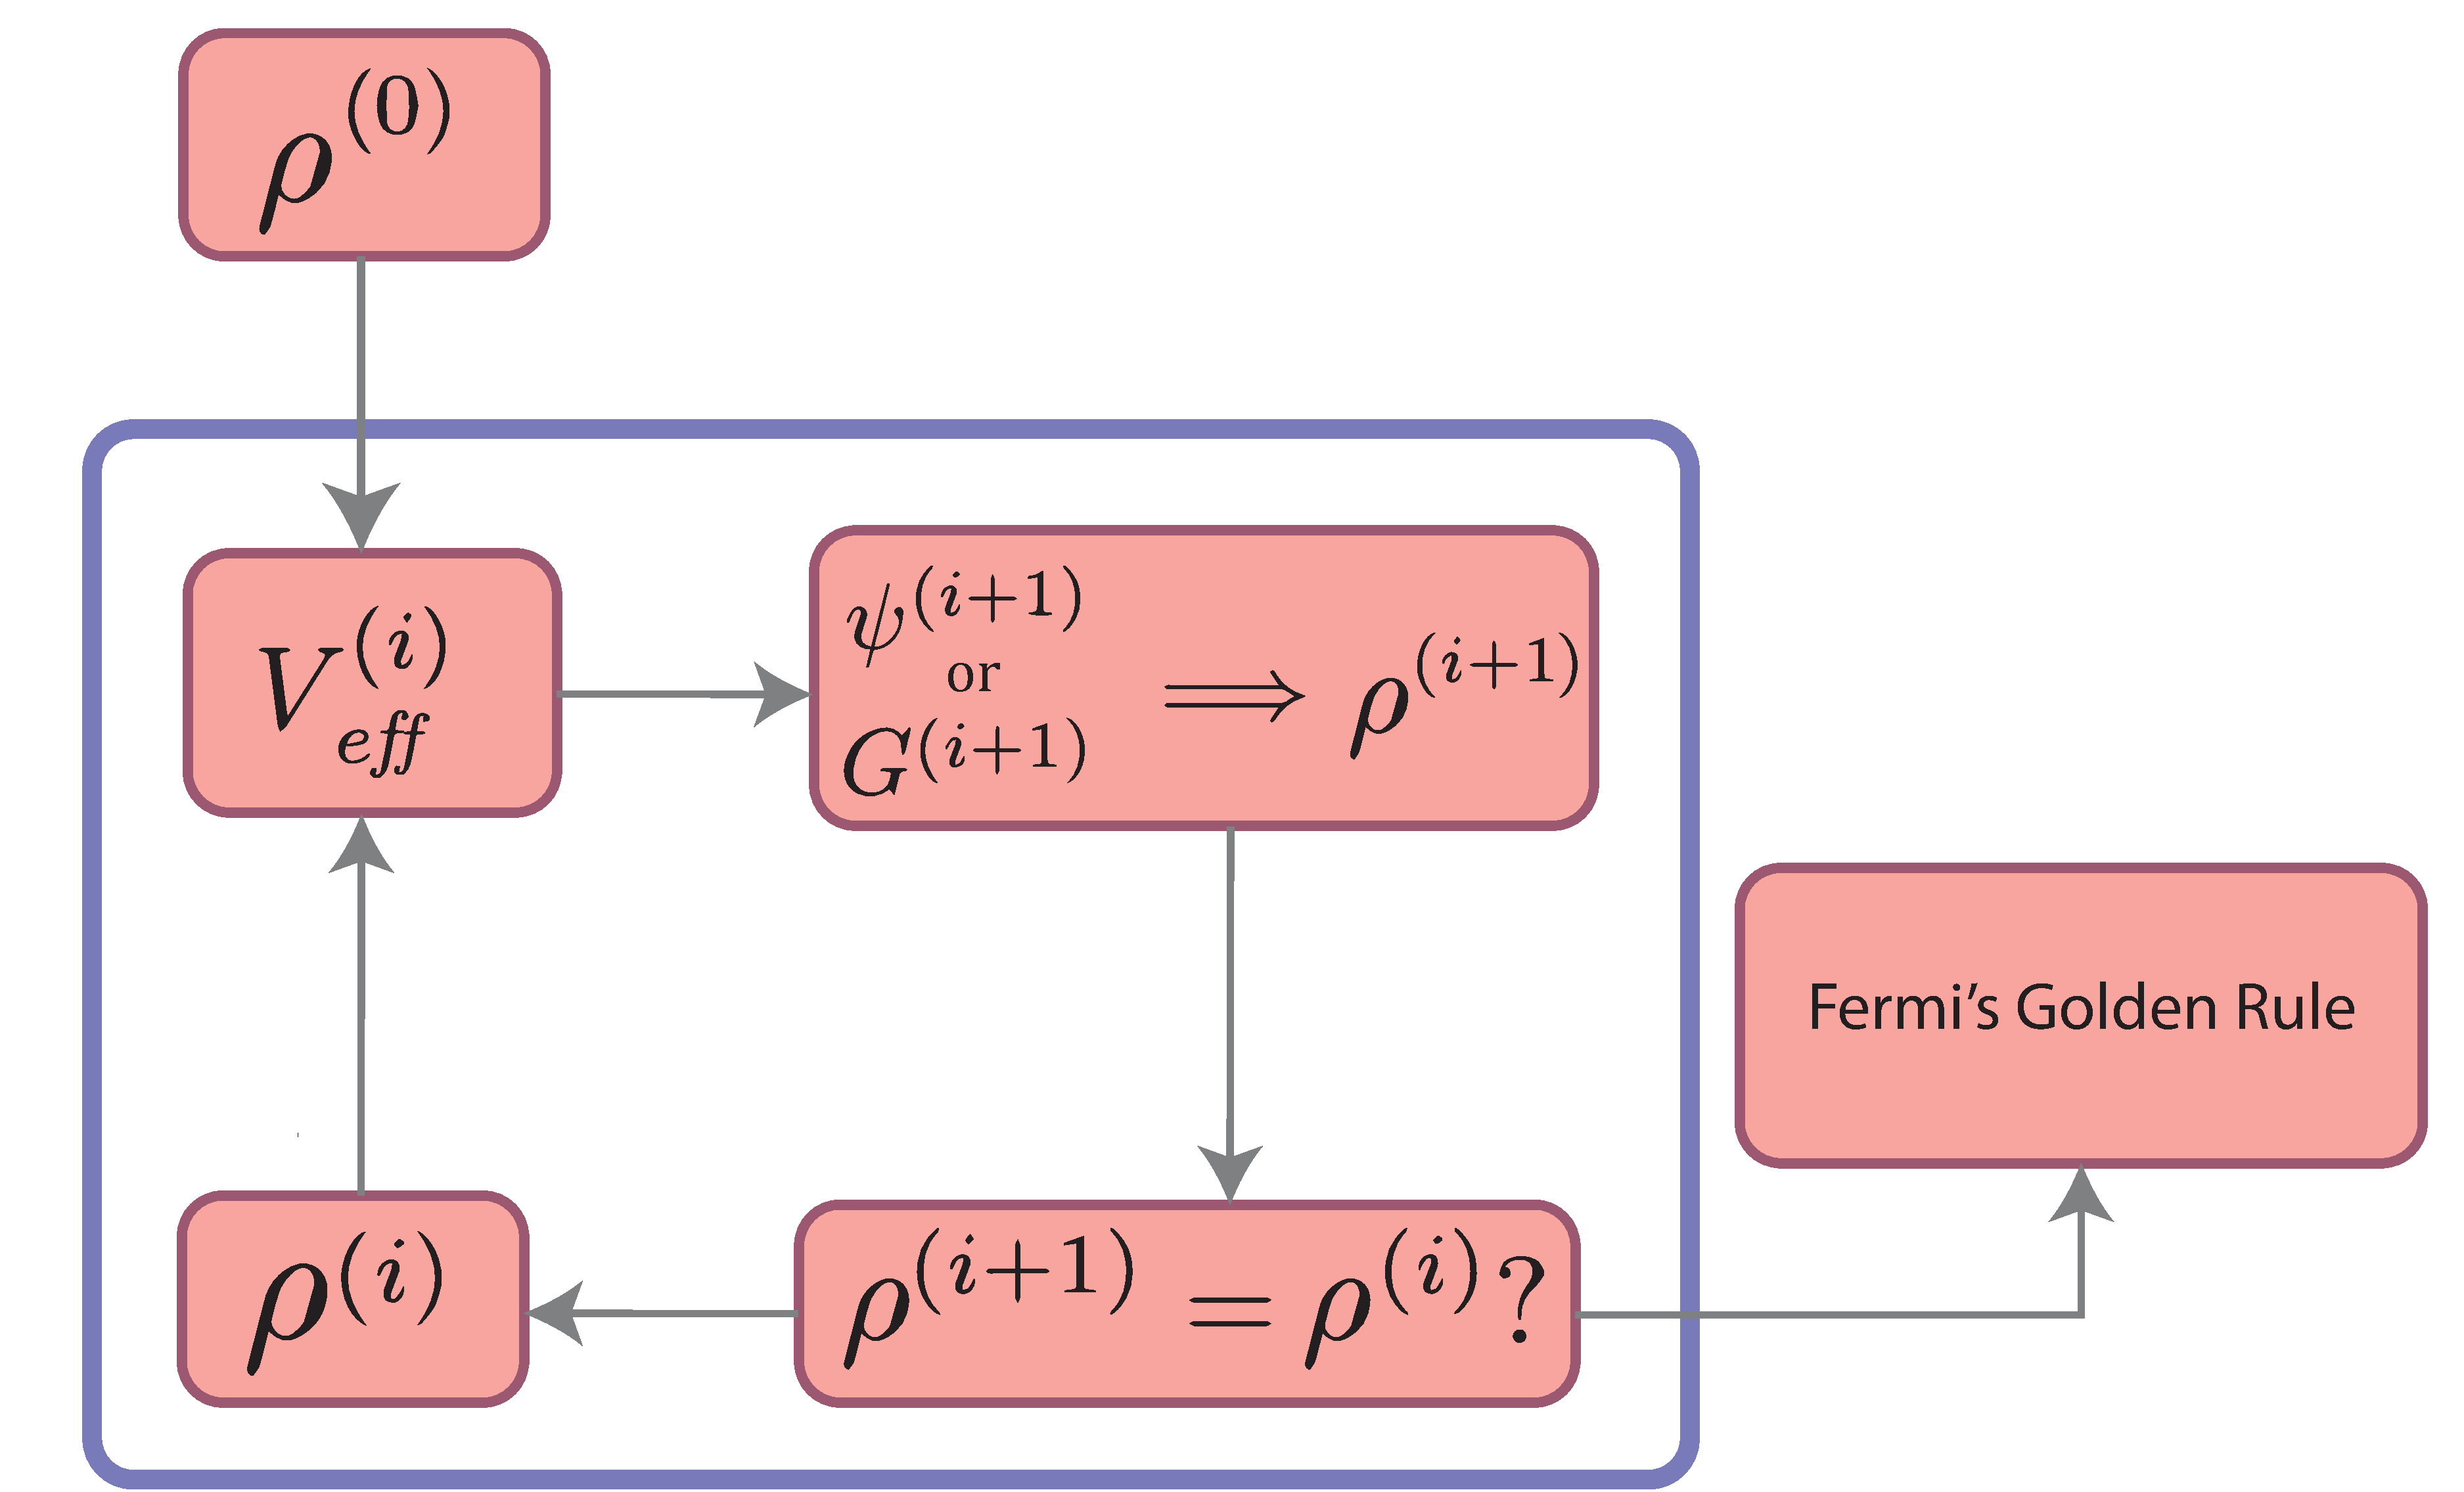
\includegraphics[width=\linewidth]{Chapters/Figures/dft-feff-diagram.pdf}
    \caption[FEFF Diagram]{Feff Diagram works by starting with an initaly guess for the density and calculating a resulting potential. From this, either the Schrodinger or Green}
    \label{fig:feff-dft-diagram}
\end{figure}

FEFF first makes an initial guess for the electronic density, $ \rho^{(0)}, $  then calculates the initial potential, $ V_{eff}^{(i)} $, which is a functional of that density. Using this potential, FEFF either solves the Schr{\"o}dinger equation or the Green's function \cite{greens-function-xafs-2021}. Finally, using the Green's function, FEFF calculates the new potential, $ \rho^{(i+1)} $, and checks if the potential is self-consistent. If not, the potential is updated, and the iterative process repeats. Once self-consistency is achieved, FEFF uses the potential to calculate the absorption spectrum using Fermi's Golden Rule \ref{FermisGoldenRule}. Alternatively, if using Green's function, FEFF calculates the density from the Green's function and solves for the absorption through a series of approximations \cite{feff-citation} \cite{rehr2010parameter}. The exact mathematical formalism is beyond the scope of this thesis.

The different calculations for FEFF are executed by a series of sub-programs, coordinated to run in order through a BASH script. The input file (typically $\texttt{FEFF.inp}$) is written by the user. The card parameters are discussed in the next section. The $\texttt{FEFF.inp}$ file is first read by the program $\texttt{rdinp}$ and the \textit{ab initio} Debye-Waller factor is calculated by $ \texttt{dmdw} $ if an optional matrix is specified \cite{feff-dw}. Then, the muffin tin (overlap) potentials are calculated via $\texttt{potph}$. FEFF calculates the free atom potentials via a relativistic Dirac-Fock model \cite{feff-dirac-fock}. Then Hedin-Lundqvist/Quinn self-energy is used for calculating the excited states, and the scattering potentials are calculated by overlapping the individual, muffin tin, and free atom densities \cite{rehr2009ab}. The last program run for the self-consistency scheme is $ \texttt{pot} $. The core holes are calculated via $ \texttt{screen} $, the angular momentum density of states is calculated with $ \texttt{ldos} $, and $ \texttt{xsph} $ calculates the scattering phase shifts along with dipole matrix elements and the x-ray cross section \cite{feff-mean-free-path}. Finally the full muliple scattering \cite{feff-multiple-scattering} is calculated and the Green's function is obtained via $ \texttt{fms} $. The matrix elements are multiplied with results from the Green's function in $ \texttt{mkgtr} $ and the multiple scattering paths are written via $ \texttt{path} $. The effective scattering amplitutes $ f_{eff} $ (from which FEFF gets its name) and XAFS parameters for each path are calculated via $ \texttt{genfmt} $, and the $ \texttt{ff2x} $ is used to obtain the final XANES spectrum, the result of which is convolved with the many-body spectral function $ \texttt{sfconv} $ and written in the file $ \texttt{xmu.dat} $.     

\section{FEFF Cards} \label{app:feff-cards}
Calculating an absorption spectrum using FEFF9 requires an input file which is comprised of the coordinates of the structure as well as a series of parameters known as cards. Extensive explanations for each card can be found in the FEFF manual \cite{rehr2010parameter}. Here, we present only a brief description and suggestions for how to alter the cards in order to help find the best parameters for replicating an experimental spectrum.  The $ \texttt{SCF} $  card helps FEFF find the self-consistency potential and better estimate the Fermi level. The $ \texttt{EDGE} $ card specifies which edge to simulate. In our case, we are interested in the $L_3$ edge. The $ \texttt{EXCHANGE} $ card specifies the exchange correlation potential used for both the fine structure and background calculations. Setting $ \texttt{S02} $ to 1 merely alters the amplitude of the absorption spectrum via $ S_0^2 $, the squared determinant of overlap integrals for core orbitals \cite{rehr2010parameter}. The amplitude can be adjust later on, hence, a large value such as one is just used by convention. The $ \texttt{XANES} $ card's parameters are all optional, but can be used to alter the output energy mesh. We select parameters that include a greater density of measurements near the regions of greatest change (the peaks). The $ \texttt{FMS} $ card provides information about the full multiple scattering. Finally, the $ \texttt{POTENTIAL} $ card describes the elements present in the material. One absorber potential must be specified as zero, while the other non-absorbing potentials are labeled with ones. Other non-absorbing elements present in the sample would be labeled as 2, 3, 4, and so on.


% SCF 4.6 0 30 .5 1
% 		EDGE    L3
% 		EXCHANGE    5   0.2 0.5
% 		S02 1.
% 		XANES   3.7 0.05    0.1
% 		FMS 7
	
% 		POTENTIALS
% 		0	79	Au	-1	-1	0.
% 		1	79	Au	-1	-1	0.

% that includes inelastic losses, self-energy effects, and vibrational
% damping.

% https://iopscience.iop.org/article/10.1088/1742-6596/430/1/012001/pdf  and that lecture on FEFF
